\newcommand{\scaler}{0.6}
\newcommand{\plytawidth}{10cm*\scaler}
\newcommand{\plytalength}{2.5cm*\scaler}
\newcommand{\plytaheight}{5cm*\scaler}
\newcommand{\railcoor}{2cm*\scaler}
\newcommand{\railwidth}{0.4cm*\scaler}
\newcommand{\railheight}{0.6cm*\scaler}
\newcommand{\xots}{0.5cm*\scaler}
\newcommand{\eots}{0.15cm*\scaler}
\newcommand{\diagox}{0.1cm*\scaler}
\newcommand{\pressx}{1cm*\scaler}
\newcommand{\pressy}{0.5cm*\scaler}
\newcommand{\diagx}{0.15cm*\scaler}
\newcommand{\diagy}{0.15cm*\scaler}
\newcommand{\stalplytax}{0.2cm*\scaler}
\newcommand{\stalplytay}{1.5cm*\scaler}
\newcommand{\arrowlength}{0.6cm*\scaler}
\newcommand{\newgeom}{5cm*\scaler}
\newcommand{\newgeomx}{8cm*\scaler}
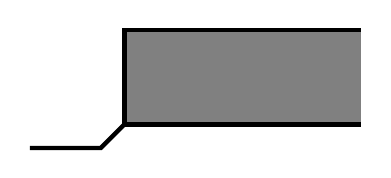
\begin{tikzpicture}
  \coordinate (A2) at (0, \pressy);
  \coordinate (B2) at (0, \plytalength);
  \coordinate (C2) at (\plytawidth/2, \pressy);
  \coordinate (D2) at (\plytawidth/2, \plytalength);
  \coordinate (E2) at (-\railcoor,  0);
  \coordinate (F2) at (-\railcoor, \plytalength);
  \coordinate (H2) at (- \pressy,  0);
  \coordinate (G2) at (\plytawidth + \pressy,  0);
   
  \draw [ultra thick, fill=gray] (C2) -- (A2) -- (B2) -- (D2);
  \draw [ultra thick] (E2) -- (H2) -- (A2);
  
\end{tikzpicture}